\documentclass[11pt, oneside]{article}   	% use "amsart" instead of "article" for AMSLaTeX format
\usepackage{geometry}                		% See geometry.pdf to learn the layout options. There are lots.
\geometry{letterpaper}                   		% ... or a4paper or a5paper or ... 
%\geometry{landscape}                		% Activate for for rotated page geometry
%\usepackage[parfill]{parskip}    		% Activate to begin paragraphs with an empty line rather than an indent
\usepackage{graphicx}				% Use pdf, png, jpg, or eps� with pdflatex; use eps in DVI mode
								% TeX will automatically convert eps --> pdf in pdflatex		
\usepackage{amssymb}
\usepackage{amsmath}
\usepackage{parskip}
\usepackage{color}

\title{Ellipse-parametrization}
%\author{The Author}
%\section{}
% \subsection*{R code}
\date{}							% Activate to display a given date or no date

\graphicspath{{/Users/telliott_admin/Dropbox/Tex/png/}}

% \begin{center} 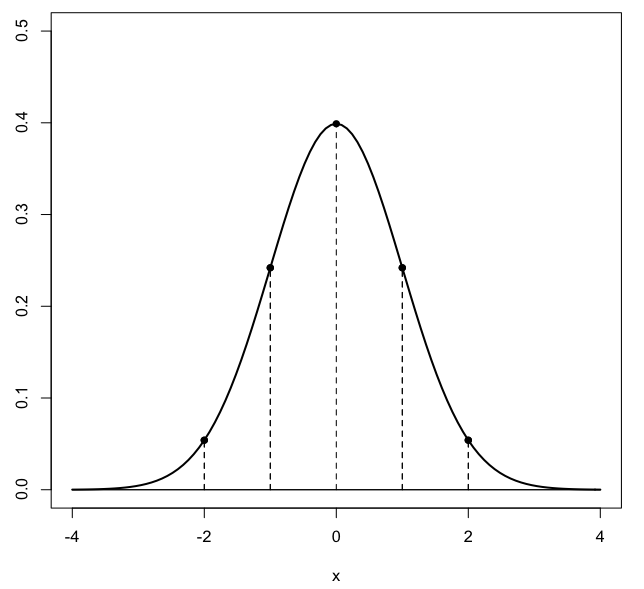
\includegraphics [scale=0.4] {gauss3.png} \end{center}
% \begin{bmatrix} a  &  b \\ c  &  d \end{bmatrix}
% \bigg |_

\begin{document}
\maketitle
\Large
%\noindent

\begin{center} 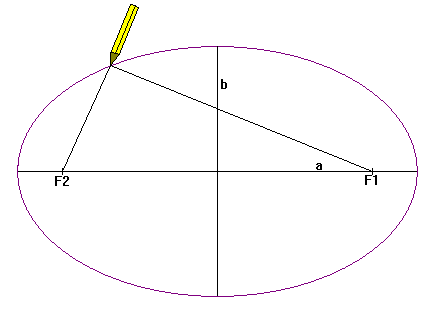
\includegraphics [scale=0.5] {ellipse_draw.png} \end{center}

Learning how to draw an ellipse using two pins and a circular string holding a pencil is an early adventure in mathematics.  The ellipse is the set of all points whose combined distance to the two pins (foci) is the same.

\begin{center} 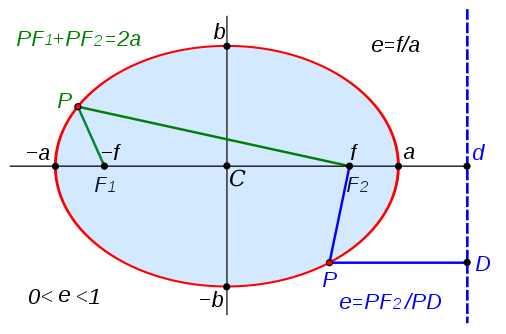
\includegraphics [scale=0.5] {ellipse_wikipedia.png} \end{center}

The pin positions with respect to the origin or center are called the foci, lying at the points ($\pm f,0$).  The lengths of the axes (called semi-major and semi-minor) are usually labeled $a$ and $b$.  Consider the situation when the pencil is at the point $(0,a)$.  The length $L$ of the string is equal to twice the distance to the left focus, $L = 2(f+a)$, so

\[ a = \frac{L}{2} - f \]

We learn in algebra that the equation for an ellipse is
\[ \frac{x^2}{a^2} + \frac{y^2}{b^2} = 1 \]

Here are three ellipses drawn with the same center.

\begin{center} 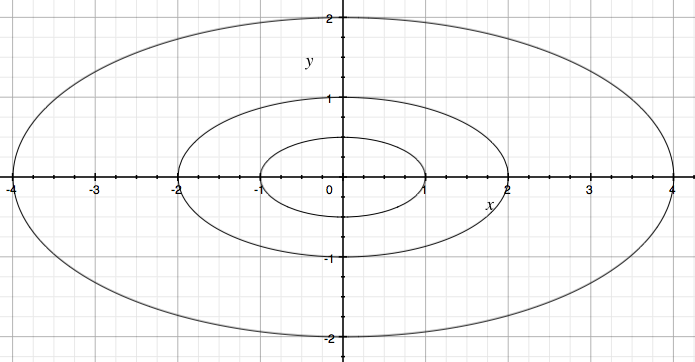
\includegraphics [scale=0.5] {ellipses_three.png} \end{center}

They were drawn by adjusting the value on the right-hand side of the equation

\[ \frac{x^2}{a^2} + \frac{y^2}{b^2} = r^2 \]

where $r = \{ 1/2,1,2 \}$.  This is equivalent to scaling both $a$ and $b$ by the same factor of $r$

\[ \frac{x^2}{(ra)^2} + \frac{y^2}{(rb)^2} = 1 \]

When $r=2$ we need to make the string a bit less than twice as long, because the length $f$ is also involved:

\[ ra = r(\frac{L}{2} - f) \]

\subsection*{parametrization}

An alternative view is the one below, which shows (black curves) the upper half of two circles of radius $r=1$ and $r=2$ and an ellipse whose equation is 
\[ \frac{x^2}{2^2} + \frac{y^2}{1} = 1 \]

\begin{center} 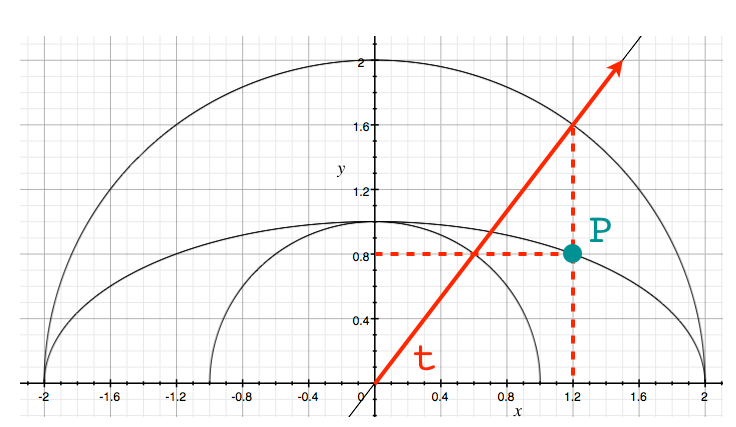
\includegraphics [scale=0.5] {p_ellipse.png} \end{center}

Here $a=2$ and $b=1$.

The standard parametrization of the ellipse is
\[ x = a \cos t \]
\[ y = b \sin t \]
which I had trouble visualizing, until I drew the picture.  The point is that the parameter $t$ is \emph{not} the angle that a ray to $P$ makes with the $x$-axis, as it is for the circle.  Instead, to find the $x$ value of $P$ corresponding to $t$, we extend the ray with angle $t$ to the larger circle, with radius $a$, where we read off the $x$-value as 
\[ x=a \cos t \]
We go back to find the intersection of the same ray with the small circle to get 
\[ y = b \sin t \]

The algebraic way to do this is to show that the parametrization is equivalent to the original formulation
\[ x^2 = a^2 \cos^2 t \]
\[ y^2 = b^2 \sin^2 t \]
\[ \frac{x^2}{a^2} + \frac{y^2}{b^2} = \cos^2 t + \sin^2 t = 1 \]
as expected.

\subsection*{rotation}

Let's return to the diagram of the ellipse with two bounding circles of radius $a$ and radius $b$.  I have a new diagram on the next page.

Consider the coordinates of the point $P=(x,y)$ (the red dot in the first quadrant) as functions of the angle $t$.  As we said, $t$ is \emph{not} the angle of a ray from the origin to $P$.

Let's draw a ray (blue dotted line) from the origin that does have angle $t$ with the $x$-axis.  How to find $x$ and $y$ from the diagram.  For $x$, extend the ray to the outer circle.  The radius is $a$, the angle is $t$, and

\[ a \cos t = x \]

This is the parametrization of the ellipse introduced above.

\begin{center} 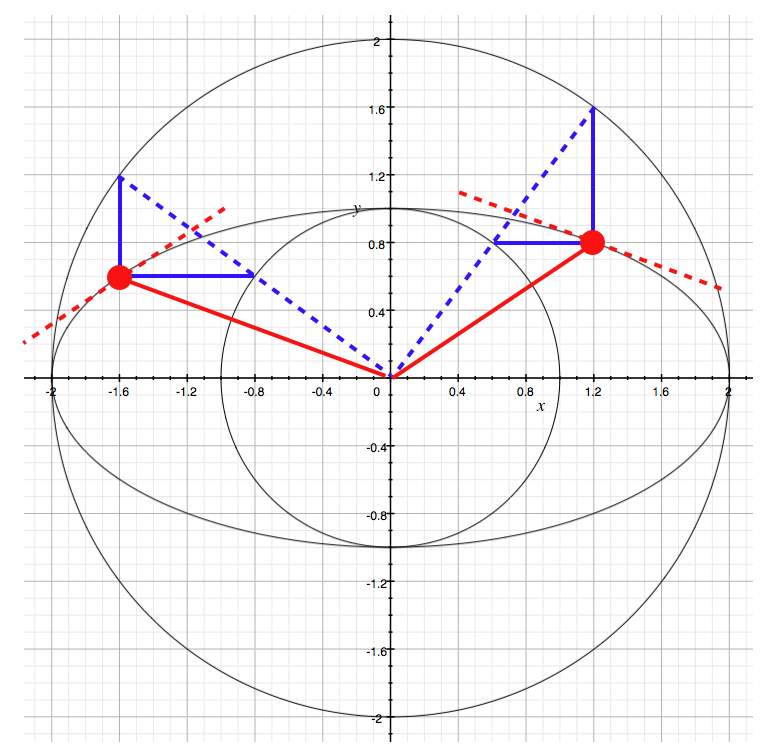
\includegraphics [scale=0.5] {ellipse_fancy.png} \end{center}

The ray drawn with angle $t$ has the same $x$-intercept with the outer circle as our point $P$ on the ellipse.  Similarly, the intercept of the ray with the inner circle has the same $y$-value as the point $P$ on the ellipse.

We estimate the point $P=(1.2,0.8)=(6/5,4/5)$.  Using our algebraic equation:

\[ \frac{x^2}{a^2} + \frac{y^2}{b^2} = 1 \]

Recall that $a=2$ and $b=1$ so

\[ x^2 + 4y^2 = 4 \]

Plugging in for $x^2$ and $y^2$ we get

\[ \frac{36}{25} + 4 \ (\frac{16}{25}) = \frac{100}{25} = 4 \]

as expected.  Reading off the intercepts for the ray with angle $t$ (dotted blue line) with the outer circle, we have the point $(1.2,1.6)$ at a distance $2$ from the origin.  Thus,

\[ \frac{1.2}{2} = 0.6 = \cos t \]
\[ t \approx 0.927\ \text{rad} \approx 53^{\circ} \]

Looking again at the figure, we want to consider what happens for the angle $u = t + \pi/2$.  This is the dotted blue ray in the second quadrant.

We might calculate the values of sine and cosine for $u$, but notice that if we view $u$ as a vector, its \emph{dot product} with $t$ must be equal to zero.  The coordinates of the intercept of the rotated vector with the outer circle are $(-1.6,1.2)$, so the cosine of the angle $u$ is

\[ \cos u = -0.8 \]
\[ u \approx 2.498 = t + \frac{\pi}{2} \ \text{rad} \approx 143^{\circ} \]

We confirm that 

\[ 2.498 - 0.927 = 1.57 = \frac{\pi}{2} \]

The coordinates of the point on the ellipse are $(-1.6,0.6)$, which we check against the formula

\[ x^2 + 4y^2 = 4 \]
\[ (1.6)^2 + 4(0.6)^2 = 2.56 + 4(0.36) = 4 \]

(no clean fractions this for this one).

\subsection*{tangent}

Finally, and this is really the point of the write-up, the vector to the point, call it $Q$, on the ellipse (red dot in the second quadrant) is the tangent to the ellipse for the point $P$ in the first quadrant, and vice-versa.

How did this happen?  Recall what we did.  We had 

\[ x = a \cos t \]
\[ y = b \sin t \]

The rotated point $Q = (x',y')$ is

\[ x' = a \cos (t + \frac{\pi}{2}) \]
\[ y' = b \sin (t + \frac{\pi}{2}) \]

\begin{center} 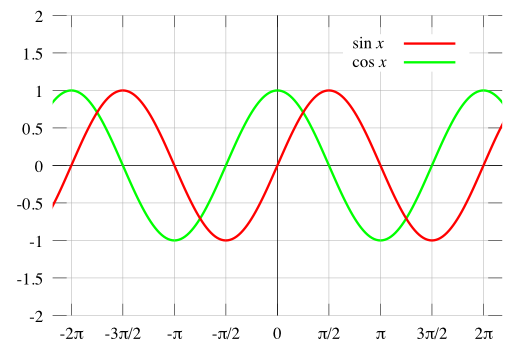
\includegraphics [scale=0.75] {sine_cosine_wikipedia.png} \end{center}

Sine is like cosine, but shifted to the right by $\pi/2$

\[ \cos \theta = \sin (\theta + \frac{\pi}{2}) \]
\[ \sin \theta = - \cos (\theta + \frac{\pi}{2}) \]

So

\[ x' = a \cos (t + \frac{\pi}{2}) = -a \sin t \]
\[ y' = b \sin (t + \frac{\pi}{2}) = b \cos t \]

So what, you say.  Well, let's look at the position vector, which can be written $\mathbf{r}(t)$, since it's a function of the angle $t$ or the time, but we will just use $\mathbf{r}$.  It has components $x$ and $y$.

\[ \mathbf{r} = \ \langle x,y \rangle \ = \ \langle a \cos t,b \sin t \rangle \ \]

Now, the tangent to the ellipse is precisely the direction in which a particle at $(x,y)$ is currently moving on the ellipse.  The tangent vector points in the same direction as the velocity vector, but $\mathbf{v}$ is just the time-derivative of the position vector.

\[ \mathbf{v} = \frac{d\mathbf{r}}{dt} = \ \langle \frac{dx}{dt}, \frac{dy}{dt} \rangle \ = \ \langle -a \sin t,b \cos t \rangle = \ \langle x',y' \rangle \]

And that's the point.   :)

\end{document}  